\begin{figure}[H]
     \begin{center}
%
        \subfigure[Anger]{%
            \label{fig:fake_anger}
            
\includegraphics[width=0.25\textwidth]{fake_anger.jpg}
        }%
        \subfigure[Contentment]{%
           \label{fig:fake_contentment}
           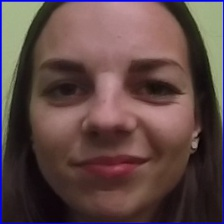
\includegraphics[width=0.25\textwidth]{fake_contentment.jpg}
        }%
        \subfigure[Disgust]{%
            \label{fig:fake_disgust}
            
\includegraphics[width=0.25\textwidth]{fake_disgust.jpg}
        }\\ %  ------- End of the first row ----------------------%
        \subfigure[Happiness]{%
            \label{fig:fake_happiness}
            
\includegraphics[width=0.25\textwidth]{fake_happiness.jpg}
        } %
        \subfigure[Sadness]{%
            \label{fig:fake_sadness}
            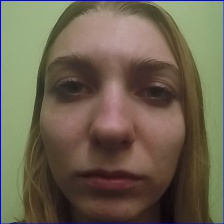
\includegraphics[width=0.25\textwidth]{fake_sadness.jpg}
        }%
        \subfigure[Surprise]{%
            \label{fig:fake_surprise}
            
\includegraphics[width=0.25\textwidth]{fake_surprise.jpg}
        }
%
    \end{center}
    \caption{%
        Six universal emotions example in Fake vs Real Expressions dataset.
     }%
   \label{fig:fakedataset_subfigures}
\end{figure}